La definición del error cuadrático medio es:
\begin{displaymath}
	ECM(\hat{\theta}) = V(\hat{\theta}) + Sesgo(\hat{\theta})^2
\end{displaymath}

Sabremos de antemano que el \textbf{E.C.M.} del estimador de momentos y el estimador de máxima verosimilitud no será cero porque sus sesgos no son nulos. Sin embargo, el \textbf{E.C.M.} del estimador de la doble mediana puede llegar a serlo si $V(\hat{b}_{med}) = 0$.

\vskip 8pt

A continuación presentamos los errores cuadráticos medios para cada estimador en función de $n$, con $n$ siendo la cantidad de muestras de tamaño $15$:

\begin{figure}[H]
	\centering
	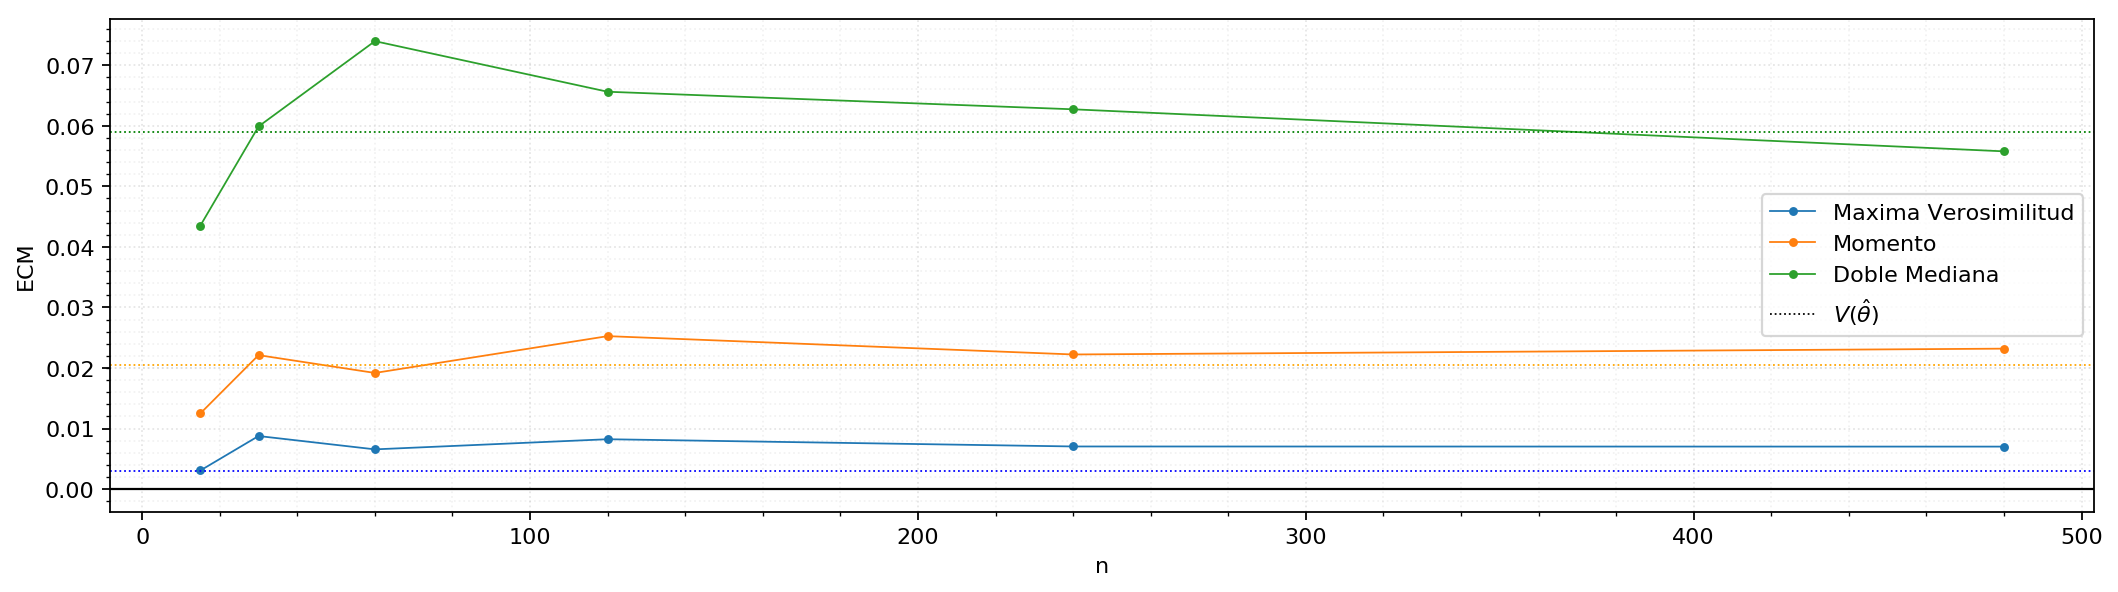
\includegraphics[width=1\textwidth]{imagenes/ecm-en-f-de-n.png}
	\caption{\footnotesize ECM de los estimadores en función de n. $a=0, b=1$}
	\label{fig:ej7-ecm-en-f-de-n}
\end{figure}

Podemos observar un pequeño indicio de tendencia hacia cero por parte del \textbf{E.C.M.} del estimador $\hat{b}_{med}$ con $n \to \infty$. Mientras tanto, la figura \ref{fig:ej7-ecm-en-f-de-n} corrobora que los errores cuadráticos medios de los estimadores $\hat{b}_{mom}$ y $\hat{b}_{mv}$ no tienden a cero.

\vskip 8pt

Ya demostramos, además, que la varianza del estimador $\hat{b}_{med}$ es cero por lo tanto es \textbf{consistente} porque su varianza tiende a cero y su esperanza al valor estimado $b$. Como los otros dos estimadores no son consistentes porque no son insesgados, nos quedamos con $\hat{b}_{med}$, cuya consistencia está asegurada.